\chapter{Design}
\label{ch:design}
\section{Introduction}
This section describes the design process of the project. There are a number of diagrams, tables, and methodologies used while designing the system. This phase is key to implementing a successful system, as it forms the basis for the implementation of the project, ensuring that the requirements of the system are met in a timely and effective manner.

\section{Technologies}
This section outlines the technologies that will be used for the project, and gives a justification for why each technology will be used. This includes programming languages, web frameworks, and libraries.

\subsection{Programming Languages}
\label{sec:lang}
Based on the research in Chapter~\ref{ch:lit}, there are a number of candidates for developing a chatbot system. Table~\ref{tab:lang} summarises the main features of each, and how they might be effective for this project.

Given the scale and scope of this project, many of the nuances and disadvantages seen in Section~\ref{sec:langreview} are irrelevant to a smaller project such as this. There appears to be libraries and frameworks in most languages that will allow the development of this system. As such, personal preference can also be considered in the choice, such as familiarity and confidence with given languages and libraries. Therefore, the project will be developed in Java, because of personal experience and familiarity with the language.

\begin{table}[h]
	\centering
	\begin{tabularx}{\textwidth}{{@{}lXXX@{}}}
		\toprule
		& Java & Python & Ruby on Rails \\
		\midrule
		Description 
			& Popular object-oriented language used in many enterprise solutions.
			& A well-established language in data science and machine learning communities.
			& Interpreted language commonly combined with Rails in web applications. \\
					\midrule
		Advantages
			& Popular language with a large community.
			
			Java Virtual Machine (JVM) allows for integrated cross-platform support.
			
			& Abundant range of libraries for machine learning.
			
			Widely used in artificial intelligence applications.
			
			& Inherently web-based, Ruby on Rails design principles such as `Convention over Configuration' allow for
			  rapid development of web applications. \\
			  		\midrule
  		Disadvantages
  			& Web-based applications require additional libraries.
  			& Not inherently web-based, although frameworks exist such as Django \cite{django2020}.
  			& Less maintainable than other web frameworks \cite{plekhanova2009evaluating}.
  			\\
  					\midrule
		Examples
			& Corpus-training an ALICE chatbot by \citet{shawar2011corpus}.
			& Chatbot techniques survey by \citet{abdul2015survey}.
			& Shopping chatbot by \citet{horzyk2009intelligent}.
			\\
  			\bottomrule
				
	\end{tabularx}
	\caption{Comparison of programming language candidates.}
	\label{tab:lang}
\end{table}

\newpage
\subsection{Libraries and Tools}
This section describes the libraries and tools required to implement the chatbot system in Java. Table~\ref{tab:libraries} describes each library and its function.

\begin{table}[h]
	\begin{tabularx}{\textwidth}{XXX}
		\toprule
		Library & Description & Link \\
		\midrule
		Spring Boot & Web framework for Java applications & \url{https://spring.io/projects/spring-boot} [Accessed 3 April 2020] \\
		\midrule
		Apache Jena & Provides functionality for SPARQL queries and linked data support & \url{https://jena.apache.org/} [Accessed 3 April 2020]\\
		\midrule
		Program AB & Provides chatbot functionality & \url{https://code.google.com/archive/p/program-ab/} [Accessed 3 April 2020]\\
		\midrule
		H2 Database & Provides database storage for the Spring Boot application & \url{http://www.h2database.com/html/main.html} [Accessed 3 April 2020] \\
		\midrule
		JUnit & Unit Testing & \url{https://junit.org/junit5/} [Accessed 3 April 2020] \\
		\bottomrule
	\end{tabularx}
	\caption{Required libraries}
	\label{tab:libraries}
\end{table}

\newpage
\section{Architecture}
\subsection{System Design}
\label{sec:systemdesign}
The overall implementation will have a number of interacting modules in order to accept user input, perform processing, and generate an output based on information from the DBPedia database. Figure~\ref{fig:design_system} provides a visual representation of this. The user input is matched against the set of chatbot AIML patterns, which determine the query requirements. The query is then built based on the values provided by the user and set by the AIML system. The SPARQL query is executed against the DBPedia live database, and the results are received and processed by the response builder. The response is displayed to the user. Although the architecture is simple, many considerations have to be made by each module, especially when dealing with users who may ask a range of questions in several different ways.

\begin{figure}[h]
	\begin{center}
		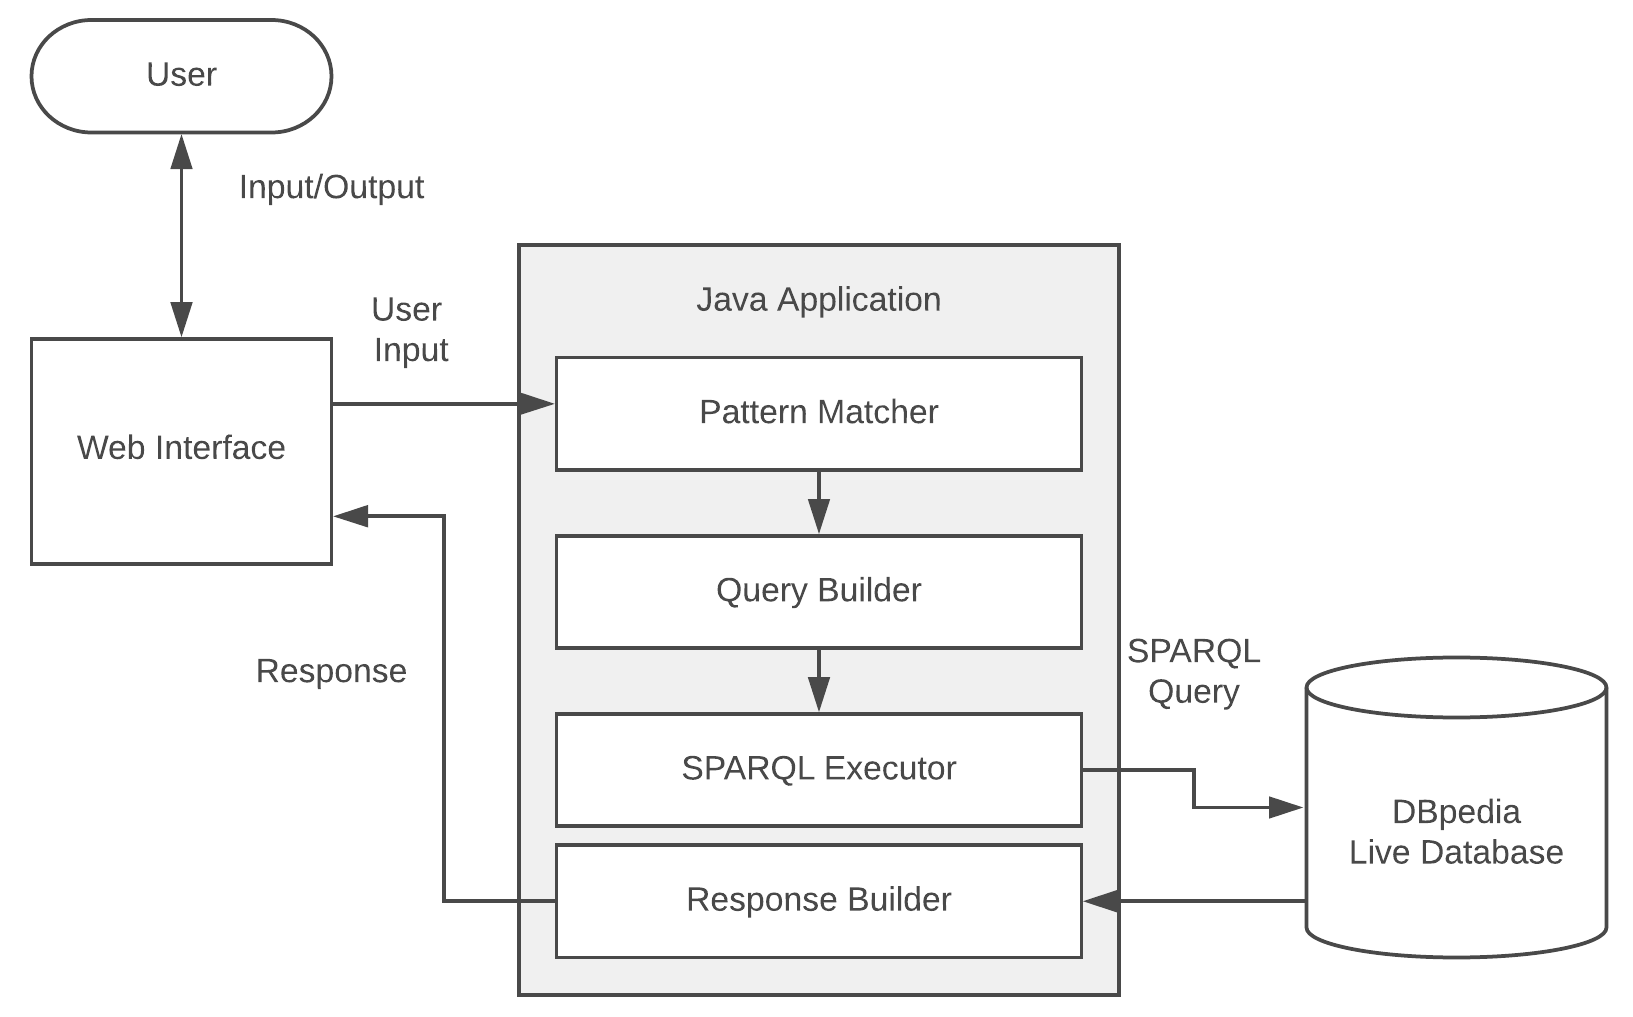
\includegraphics[width=\textwidth]{design_system}
	\end{center}
	\caption{Overview of architecture of the system.}
	\label{fig:design_system}
\end{figure}

\newpage
\subsection{Activity}
Figure~\ref{fig:design_activity} shows the flow of events through the system, from the user input to the resulting output. The activity starts in the web page, where the user inputs a query and posts it to the system. Processing of this query is performed by the Java application, which generates a query and sends it to the SPARQL endpoint. The response is received by the application, and processed into a response which is displayed in the web page.

\begin{figure}[h]
	\begin{center}
		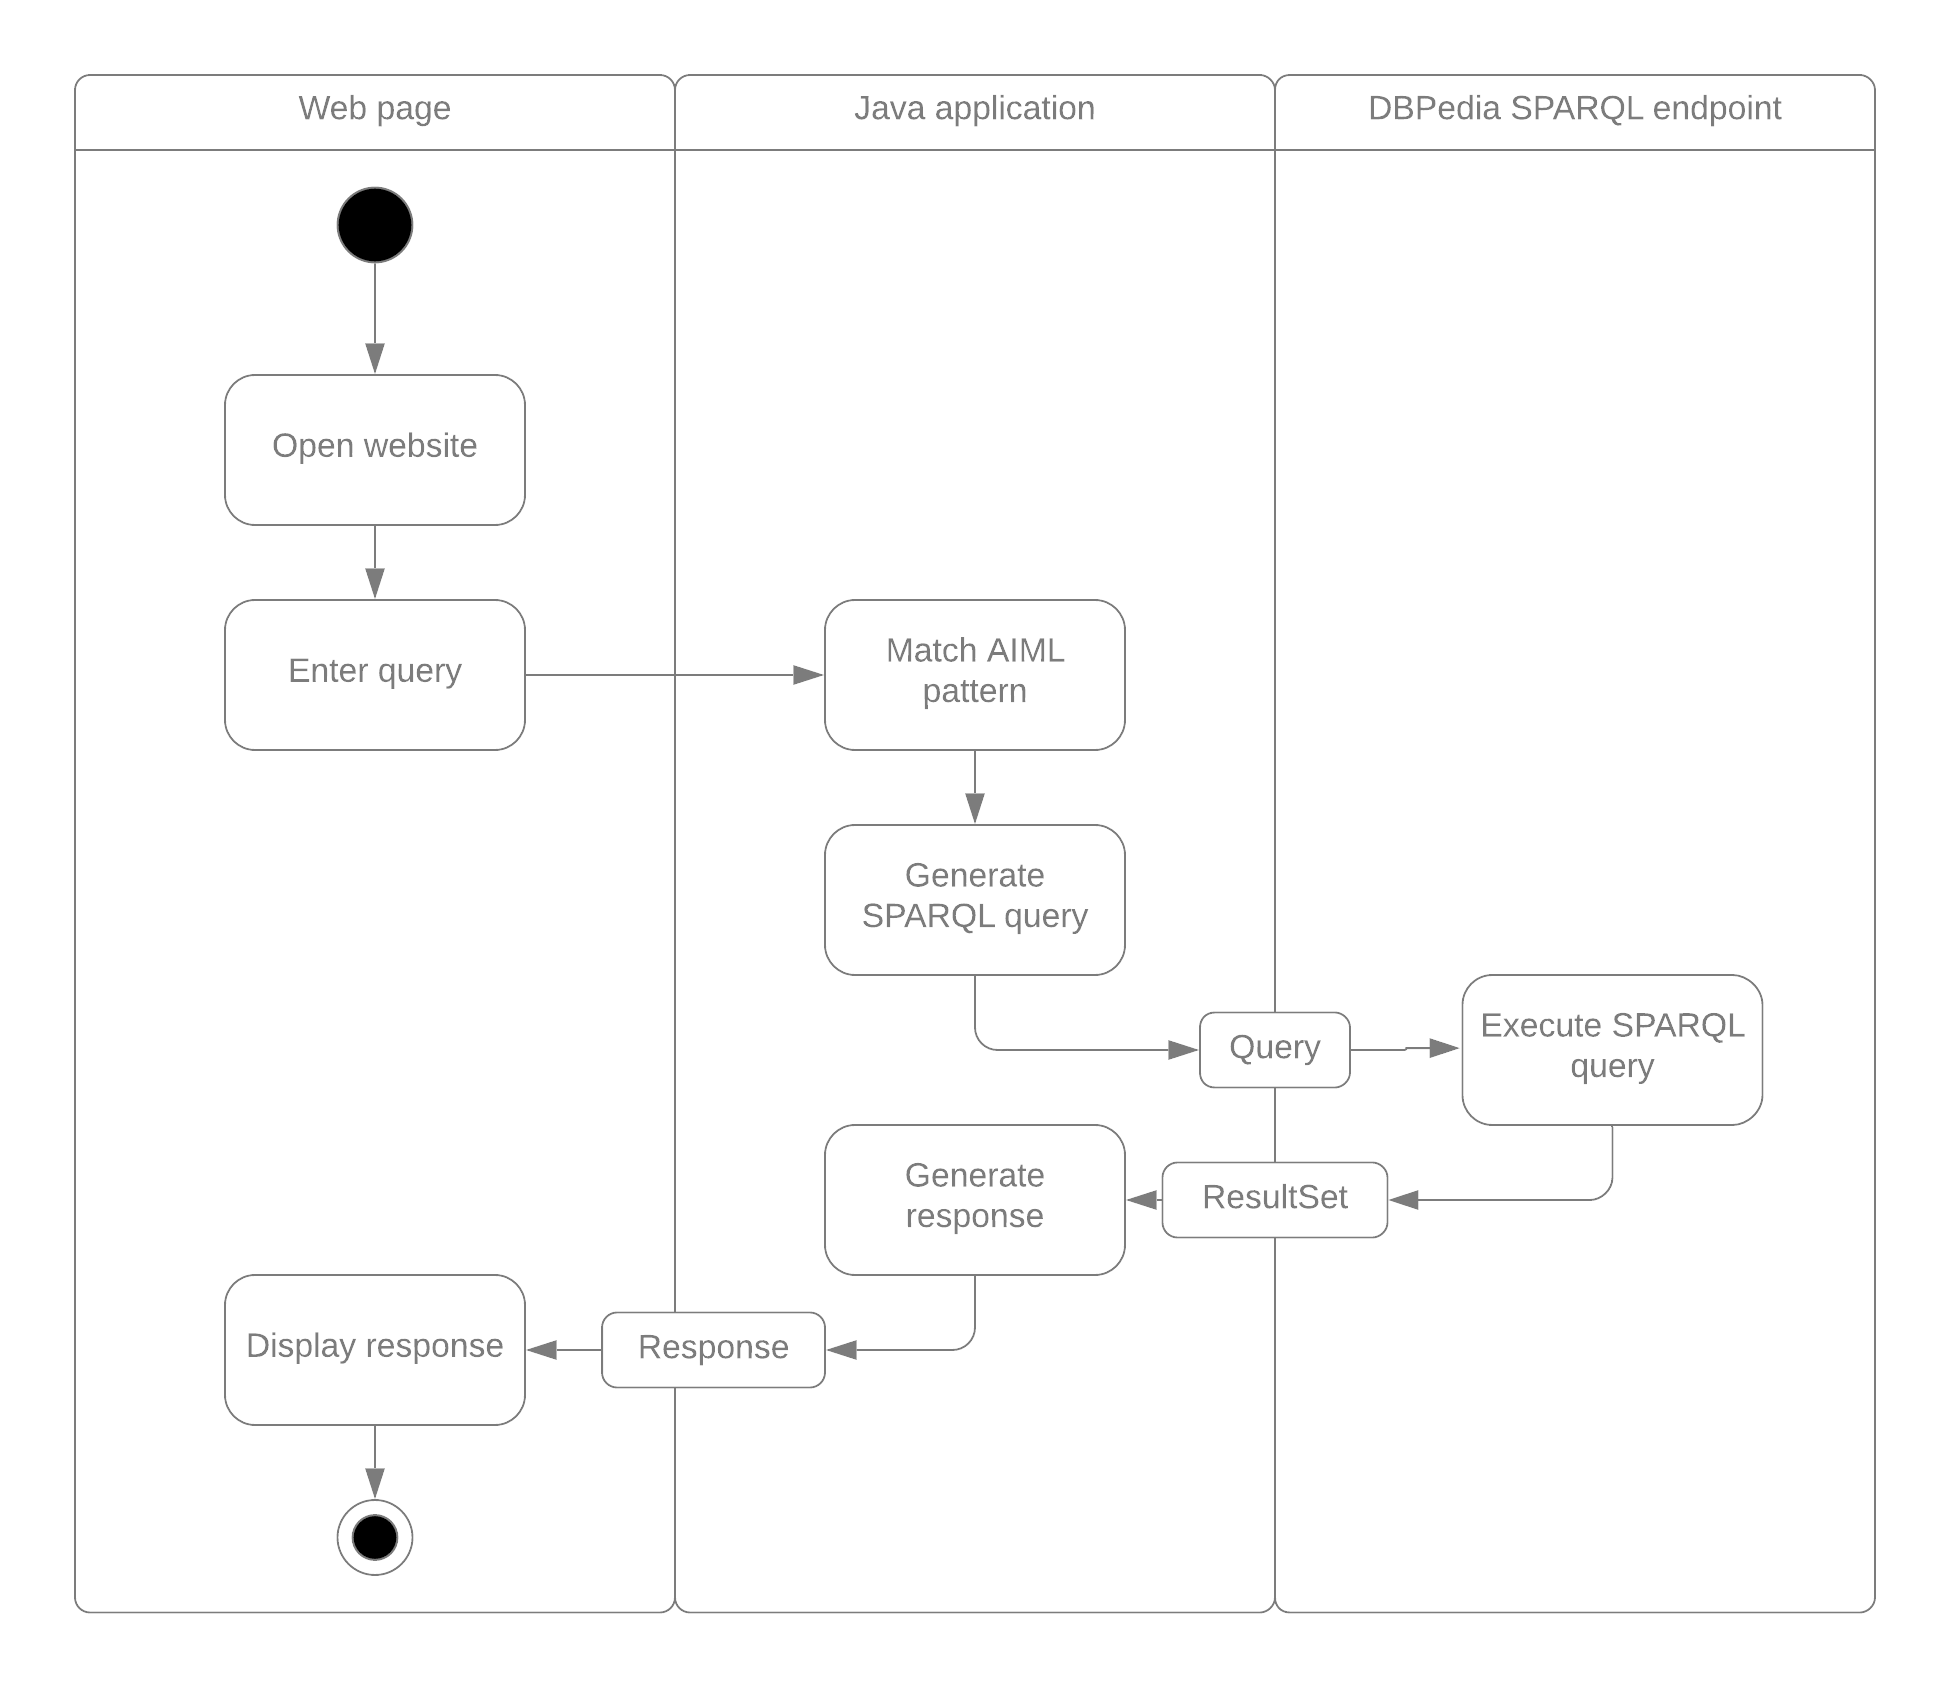
\includegraphics[width=\textwidth]{design_activity}
	\end{center}
	\caption{UML Activity diagram.}
	\label{fig:design_activity}
\end{figure}

\section{Conversation Flowchart}
One of the requirements of the system is maintaining the context of the conversation through multiple lines of dialogue. This means that if a user has asked a question about a person -- ``Who is Alan Turing?'' -- they can then ask follow-up questions, such as ``What is he known for?''. This prevents the user having to repeat the subject of each question, allowing for a more natural conversation flow. Figure~\ref{fig:flowchart} shows a flowchart for this conversation flow, and how the chatbot will set and maintain the conversation context.

\begin{figure}[h]
	\begin{center}
		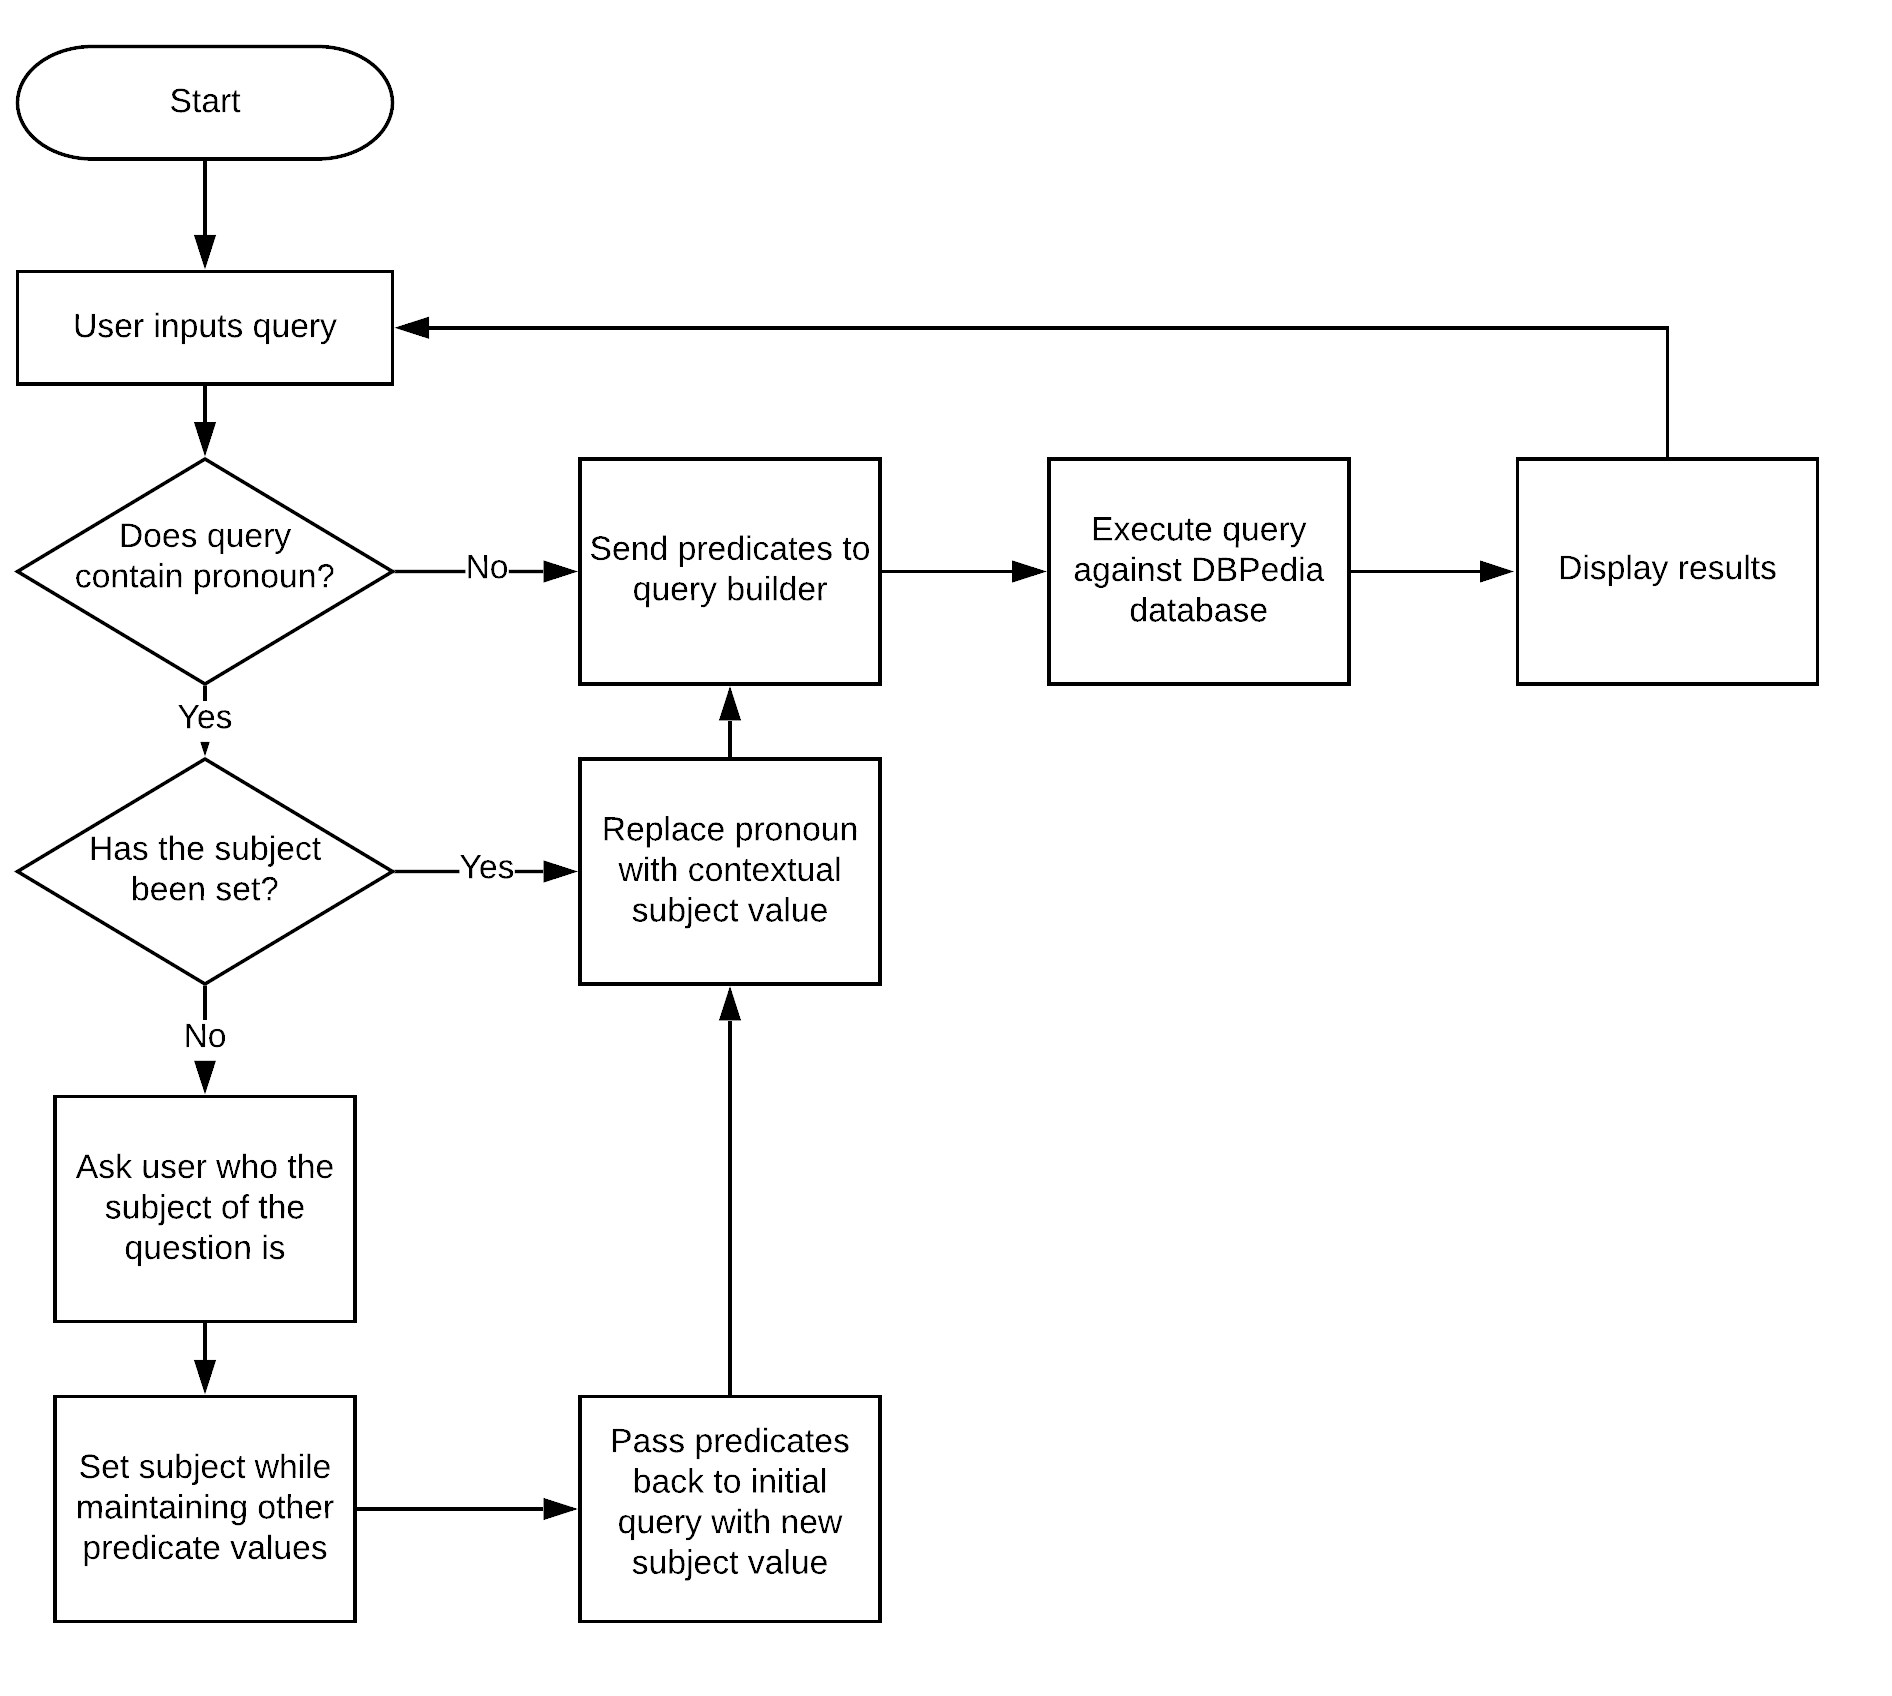
\includegraphics[width=\textwidth]{flowchart}
	\end{center}
	\caption{Conversation flowchart diagram.}
	\label{fig:flowchart}
\end{figure}

\section{Class Diagram}
This class diagram in Figure~\ref{fig:class_diagram} visualises the overall function and interoperation of the classes in the proposed system. Many of these classes are requirements for the Spring Boot application to operate. The \code{WebController} classes provides the main routing and logic of the application. The \code{MessageRepository} and \code{MessageItemRepository} act as adapters between the the Spring application and a database.

The main logic for the chatbot is held in the \code{ChatbotService} class, which links user queries with the \code{QueryBuilder} class, which generates SPARQL queries. The \code{DBPedia} class executes the queries and generates a response for the user. \code{Message} objects are used to store the content of the messages, where a \code{Message} may consist of zero or many \code{MessageItems}, in the case of list messages.

\begin{figure}[h]
	\begin{center}
		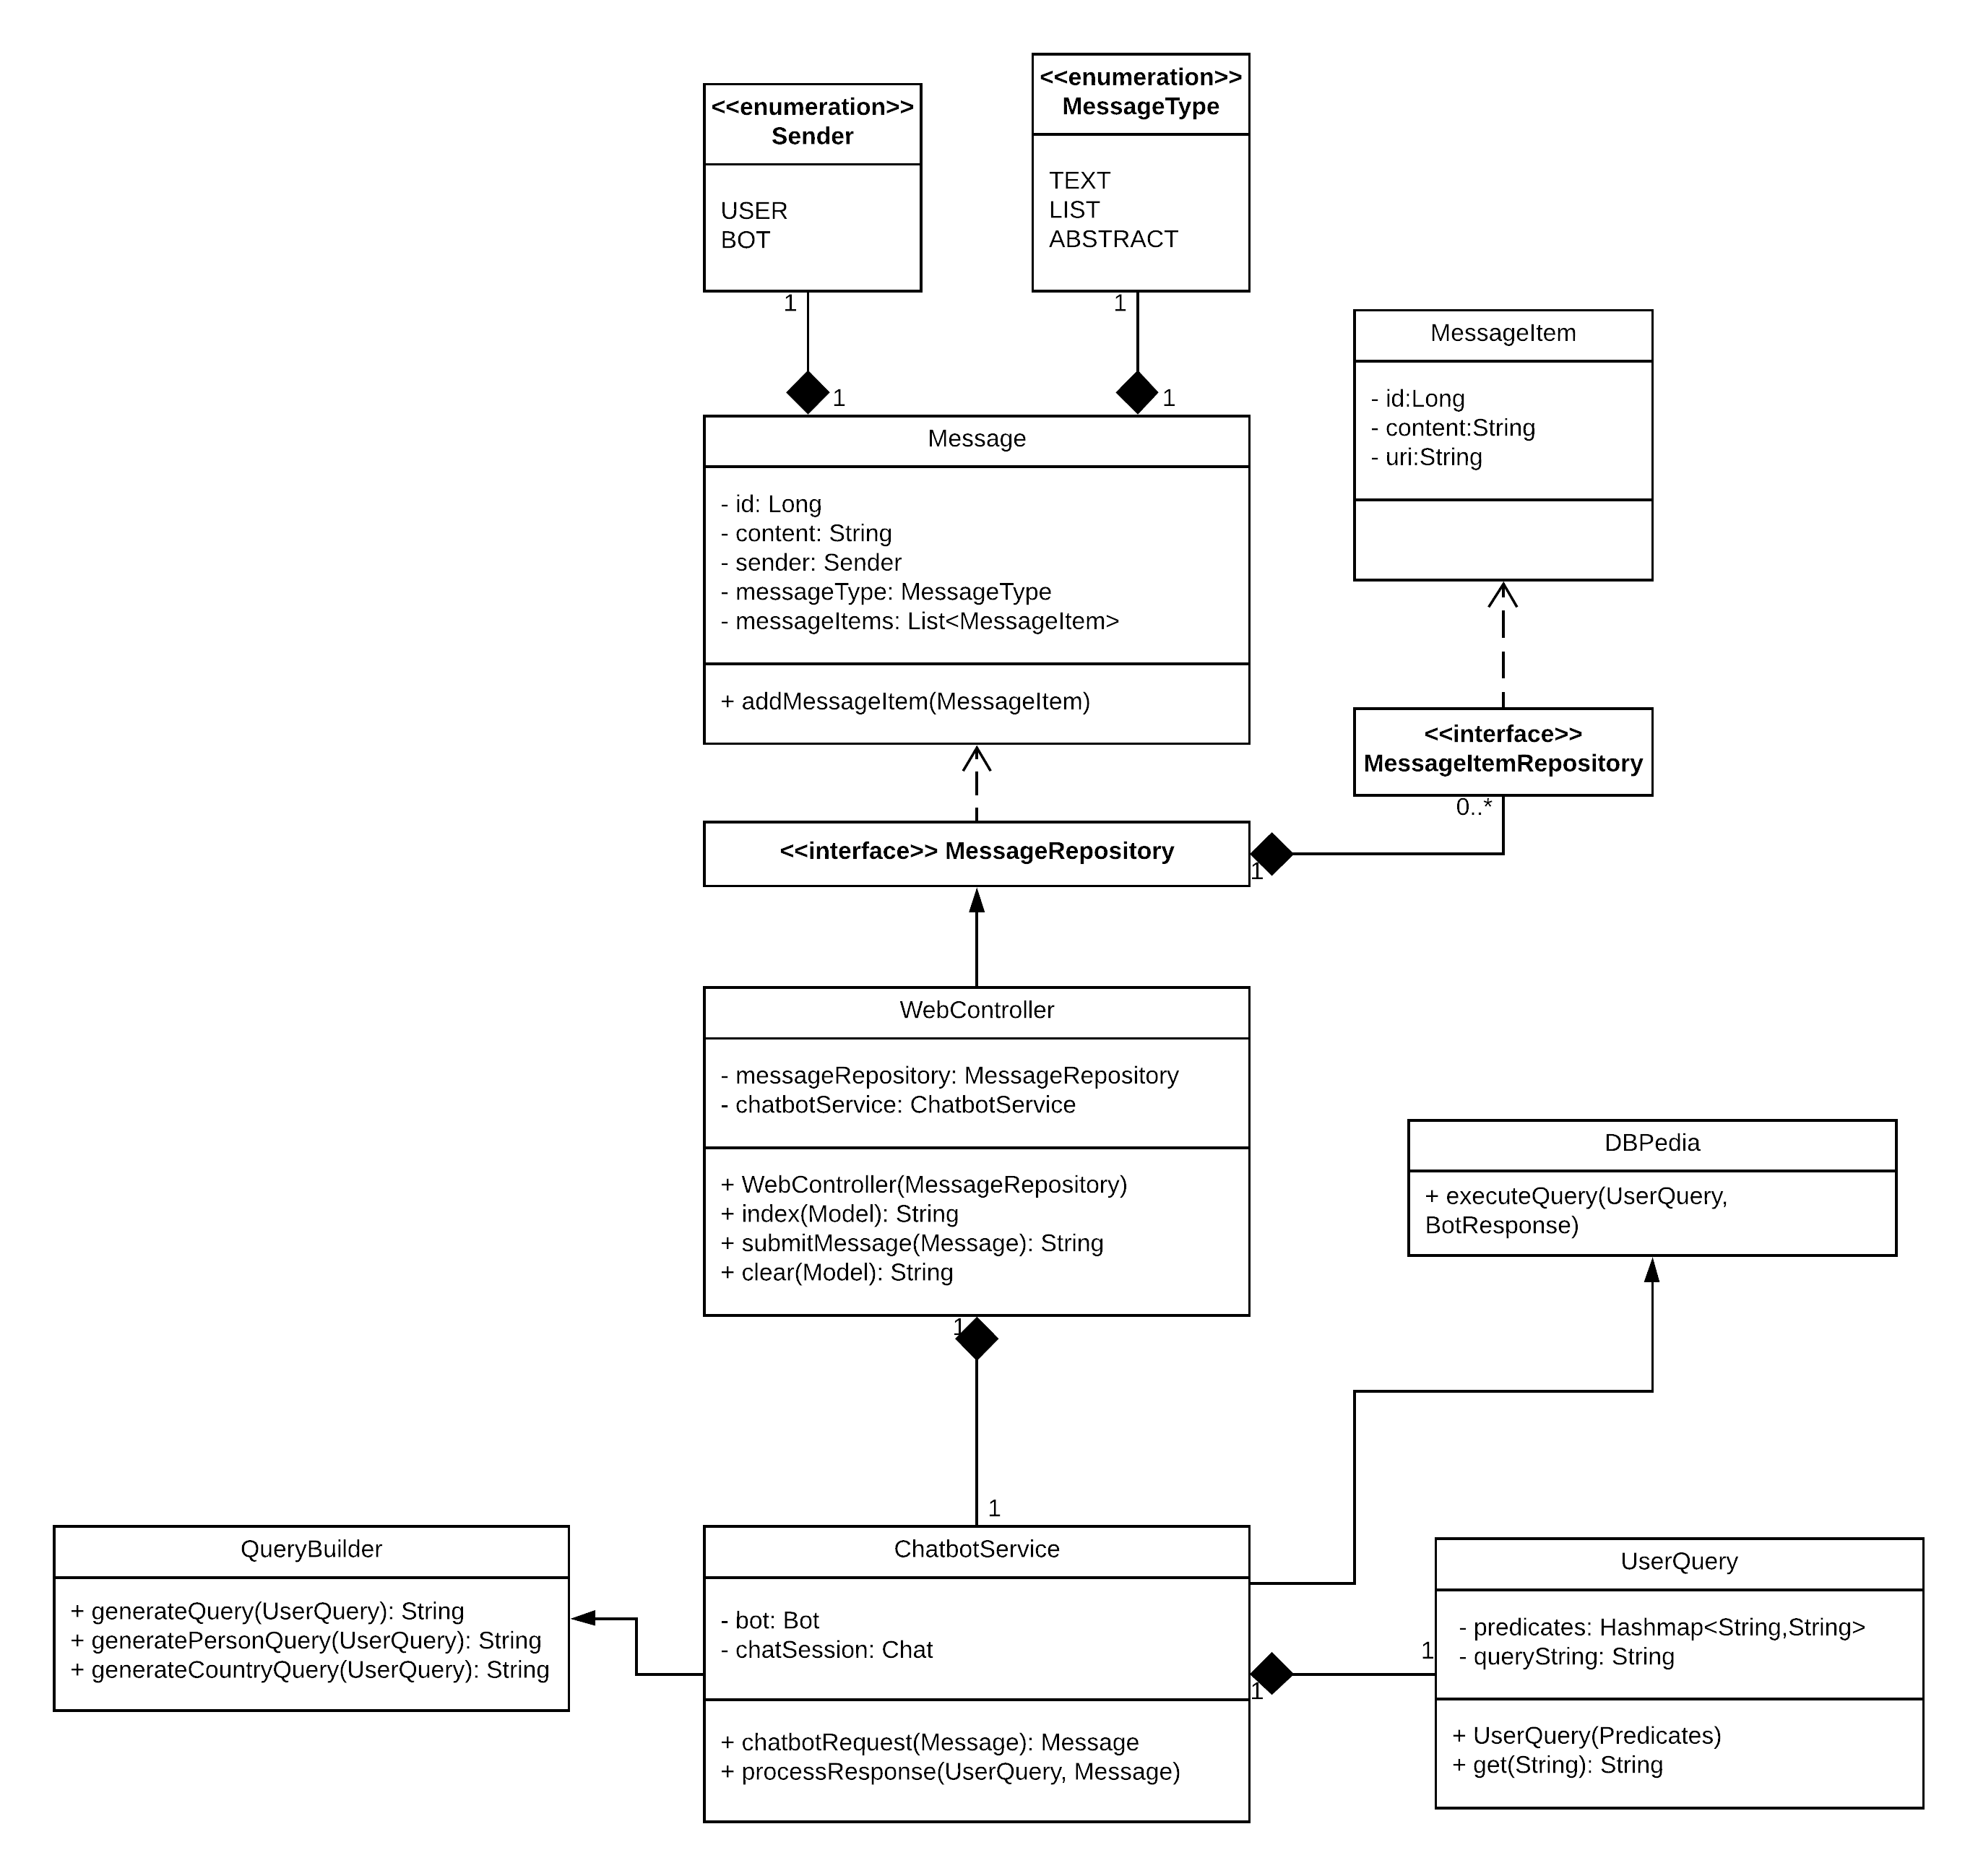
\includegraphics[width=\textwidth]{class_diag}
	\end{center}
	\caption{UML Class diagram.}
	\label{fig:class_diagram}
\end{figure}

\newpage
\section{User Interface}
The proposed system will be a web application for a number of reasons. Firstly, it will allow testers to easily access the application without having to download any files. It also allows for easy customisation using HTML and CSS. The alternative would be a text-based user interface (TUI), which would require less configuration, but will be limited in terms of rendering images, links, and other elements. It will be beneficial to use a TUI during development, as this would allow the system to be built and debugged quickly. Figure~\ref{fig:design_ui} shows the expected web interface design for the system.

\begin{figure}[h]
	\begin{center}
		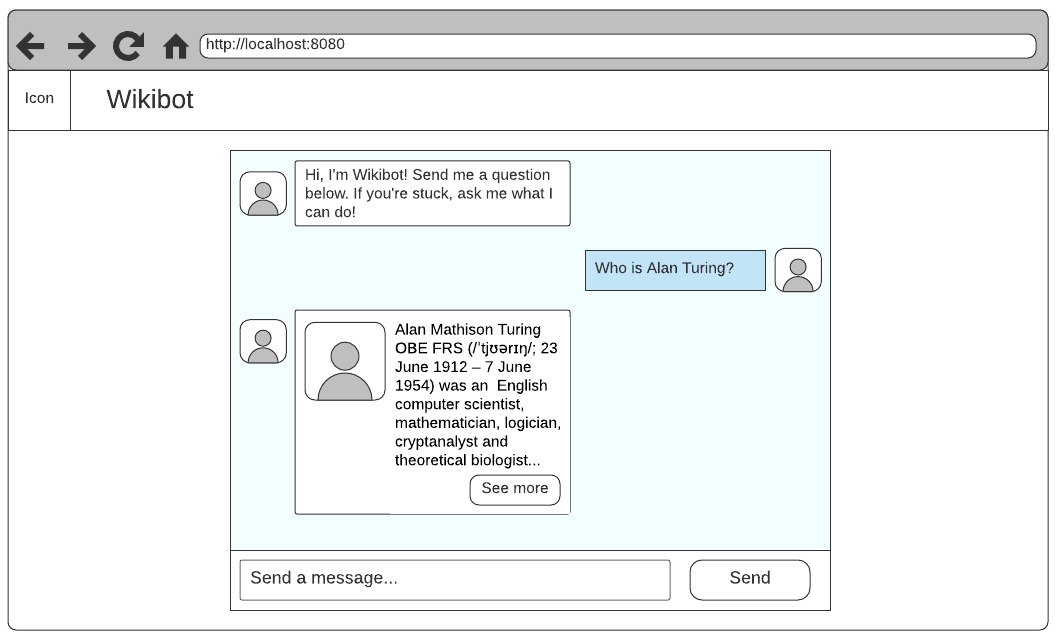
\includegraphics[width=.8\textwidth]{design_ui}
	\end{center}
	\caption{Web UI interface design.}
	\label{fig:design_ui}
\end{figure}

\section{Data}
This section discusses the data design for the system. This includes a database for storing conversations, as well as introduces the AIML pattern designs that will be required for the chatbot to match inputs to responses.

\subsection{Database}
For the chatbot to be able to maintain a conversation with the user, there must be an element of storage within the system. The storage requirements are simple, as we only need to store one entity - messages. This is because the message entity will store all of the metadata, including who sent it and its contents. Therefore, the database design shown in Figure~\ref{fig:dbdesign} is simple, and maps directly to the Message and MessageItem objects shown in Figure~\ref{fig:class_diagram}.

\begin{figure}[h]
	\begin{center}
		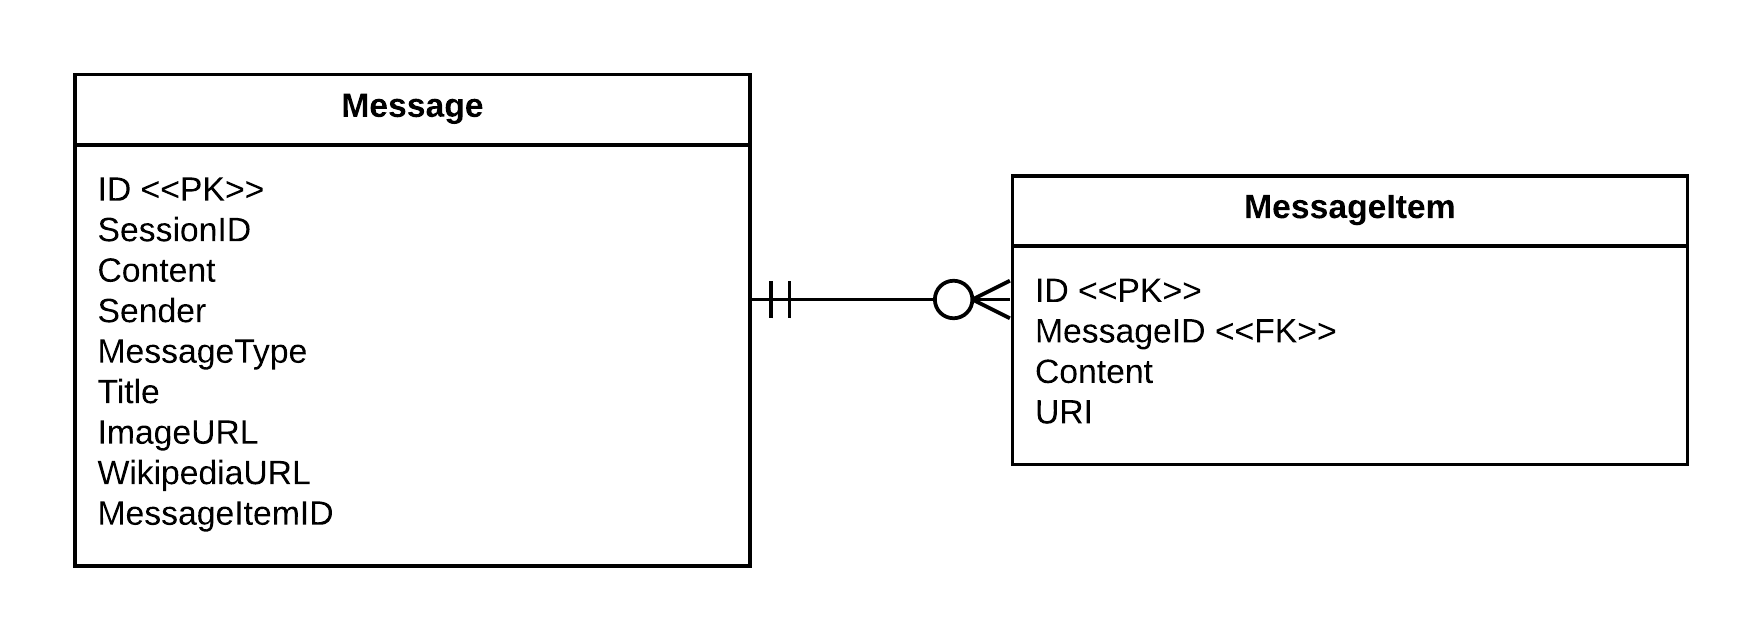
\includegraphics[width=.7\textwidth]{database}
	\end{center}
	\caption{Web UI interface design.}
	\label{fig:dbdesign}
\end{figure}

\subsection{AIML}
The majority of the conversational logic is found in the AIML patterns. This is where the user input is matched to a pattern to produce the expected result. One of the main issues to contend with here is that a user may ask a question in many different ways. For example, to meet requirement F8 (Person Age Query), the user could ask:
\begin{itemize}
	\setlength\itemsep{0em}
	\item How old is X?
	\item What is X's age?
	\item Age of X
	\item X age
\end{itemize}

Therefore, the system must be able to distinguish these phrases to match to the correct output. As such, one helpful feature in AIML is \code{<srai/>}, which allows us to link a pattern to an existing one. This prevents redundant code being added and we can add many synonymous phrases to match to the same query. Table~\ref{tab:aiml} lists some of the AIML patterns that will be required to meet the requirements identified in Section~\ref{sec:requirements}. Note that this list is not exhaustive, but will provide some direction when developing the chatbot.

\subsection{Conclusion}
This section established a thorough design document from which to implement the system. This allows us to visualise how the final system should operate, and how the user should be able to interact with the chatbot. The next section documents the planning and implementation of the project.

\newpage
\begin{table}[h]
	\centering
	\begin{tabularx}{\textwidth}{XX}
		\toprule
		Requirement & Pattern \\
		\midrule
		F6. Person Description Query & 
		\shortstack[l]{
			   \code{WHO IS *}
			\\ \code{TELL ME ABOUT *}
			\\ \code{* DESCRIPTION}
		}
		\\
		\midrule
		F7. Person Birthdate Query & 
		\shortstack[l]{
			\code{WHEN WAS * BORN}
			\\ \code{* BIRTHDATE}
			\\ \code{* BIRTH DATE}
			\\ \code{WHAT IS * DATE OF BIRTH}
		}
		\\
		\midrule
		F8. Person Age Query & 
		\shortstack[l]{
			\code{HOW OLD IS *}
			\\ \code{* AGE}
			\\ \code{HOW OLD WAS *}
			\\ \code{WHAT AGE IS *}
		}
		\\
		\midrule
		F9. Person Birthplace Query & 
		\shortstack[l]{
			\code{WHERE WAS * BORN}
			\\ \code{* BIRTHPLACE}
			\\ \code{* PLACE OF BIRTH}
		}
		\\
		\midrule
		F10. Person Death Date Query & 
		\shortstack[l]{
			\code{WHEN DID * DIE}
			\\ \code{WHAT YEAR DID * DIE}
			\\ \code{* DEATH DATE}
		}
		\\
		\midrule
		F11. Person Known For Query & 
		\shortstack[l]{
			\code{WHAT IS * KNOWN FOR}
			\\ \code{WHAT IS * FAMOUS FOR}
			\\ \code{* KNOWN FOR}
		}
		\\
		\midrule
		F12. Person Photo Query & 
		\shortstack[l]{
			\code{WHAT DOES * LOOK LIKE}
			\\ \code{PHOTO OF *}
			\\ \code{PICTURE OF *}
			\\ \code{SHOW ME A PICTURE OF *}
		}
		\\
		\midrule
		F13. Person Wikipedia Link Query & 
		\shortstack[l]{
			\code{* WIKIPEDIA}
			\\ \code{* WIKIPEDIA PAGE}
			\\ \code{LINK TO * WIKIPEDIA}
		}
		\\
		\midrule
		F14. Country Description Query & 
		\shortstack[l]{
			\code{WHERE IS *}
			\\ \code{* COUNTRY}
			\\ \code{DESCRIBE *}
		}
		\\
		\midrule
		F15. Country Population Query & 
		\shortstack[l]{
			\code{POPULATION OF *}
			\\ \code{HOW MANY PEOPLE LIVE IN *}
			\\ \code{* CURRENT POPULATION}
		}
		\\
		\midrule
		F16. Country Capital Query & 
		\shortstack[l]{
			\code{CAPITAL OF *}
			\\ \code{* CAPITAL}
			\\ \code{WHAT IS THE CAPITAL OF *}
		}
		\\
		\midrule
		F17. Person List Query & 
		\shortstack[l]{
			\code{LIST OF *}
			\\ \code{LIST OF 10 *}
			\\ \code{SHOW ME A LIST OF *}
		}
		\\
		\midrule
		F18. Person AND Query & 
		\shortstack[l]{
			\code{* BORN IN * AND *}
			\\ \code{* NAMED * AND BORN BEFORE *}
			\\ \code{* BORN IN * AND WINNERS OF *}
		}
		\\
		\midrule
		F19. Context-aware Conversation & 
		\shortstack[l]{
			\code{WHERE WAS HE BORN}
			\\ \code{WHAT IS HE KNOWN FOR}
			\\ \code{WHAT IS ITS CAPITAL}
		}
		\\
		\midrule
		F20. Chatbot Greeting & 
		\shortstack[l]{
			\code{HI *}
			\\ \code{HELLO}
			\\ \code{GREETINGS}
		}
		\\
		\midrule
		F21. Chatbot Examples & 
		\shortstack[l]{
			\code{EXAMPLES}
			\\ \code{WHAT CAN YOU DO}
			\\ \code{WHAT ARE YOUR FUNCTIONS}
		}
		\\
		\midrule
		F22. Chatbot Help & 
		\shortstack[l]{
			\code{HELP}
			\\ \code{I NEED HELP}
			\\ \code{IM STUCK}
		}
		\\
		\bottomrule
		
	\end{tabularx}
	\caption{AIML patterns matched against requirements}
	\label{tab:aiml}
\end{table}

